\section{Neural loss intervention}\label{sec:neural-information}
This separate study varies constraints, capacity and loss information
in the eight-dimensional system of Section~\ref{sec:neural-setup}, with
ball constraints. Its learned output matrix is not the fixed embedding
required by Proposition~\ref{prop:minimal-information}.

\subsection{Student}
The student is a bias-free $8\to w\to8$ SiLU network with radial
projection, $w\in\{2,4,16\}$. Actions lie in its output matrix's column
span. Width 16 can represent the target exactly by
$\operatorname{SiLU}(s)-\operatorname{SiLU}(-s)=s$, verified numerically.
Zero output weights initialize every student at the teacher; first-layer
weights are paired across losses.


\subsection{Protocol}
Up to common division by action dimension, the losses are
\begin{align}
 L_{\rm point}&=\|u-v\|^2,\\
 L_{\rm restored}&=\|u-v\|^2+(n/a)^\top(u-v),\\
 L_{\rm weight}&=(1+\|n\|/(2aR))\|u-v\|^2,\\
 L_{\rm shuffled}&=\|u-v\|^2+(n_\sigma/a)^\top(u-v).
\end{align}
The fixed random permutation $\sigma$ breaks the state--normal
association. Restoration equals Bellman regret divided by $a$;
weighting omits radial slack. At $R=32$ all normals vanish.

The initial study crosses $R\in\{0.5,2,8,32\}$, three widths, four
losses and five seeds (240 fits), with restored-minus-point at
$R=2,w=2$ as primary. Confirmation selects the initial severe-constraint
secondary condition $R=0.5,w=2$ as primary, with ten independent seeds,
$R\in\{0.5,2,32\}$, all widths and losses (360 fits). Its plan, source
hashes and seeds are frozen before training. Samples are not pooled.
Paired 95\% $t$ intervals use seed means and are not multiplicity-adjusted.

\subsection{Results}
The initial primary is inconclusive: regret difference $+0.000318$
with 95\% interval $[-0.016912,0.017548]$ and one win in five pairs.
The severe-constraint secondary improves in all five pairs at widths
2 and 4, though the width-2 interval crosses zero.

Independent confirmation at $R=0.5,w=2$ reduces normalized regret from
0.549027 to 0.448915 (18.23\%). The paired difference is $-0.100112$
$[-0.198038,-0.002185]$, with ten wins. Eight effects lie between
$-0.03884$ and $-0.03238$; two are $-0.37530$ and $-0.34355$.
The width-4 secondary also has ten wins but interval
$[-0.139534,0.002312]$.

In the confirmation primary, action MSE rises from 0.020590 to
0.022357 while the normal contribution falls from 0.047222 to
0.034574. Exact regret, their sum with MSE multiplied by $8a$, falls
from 0.062047 to 0.050671. Weight-only regret is 0.504262; restored
minus weight is $-0.055347$ $[-0.057134,-0.053560]$. Weighting achieves
smaller weighted-distance loss (0.036247 versus 0.042683) but larger
omitted slack (0.020673 versus 0.007989). Shuffled-normal regret is
0.635812, with restored-minus-shuffled difference $-0.186897$
$[-0.247484,-0.126310]$. These are post-fit decompositions, without a
claim of unique causal mediation.

At $R=32$, parameter tensors are identical across losses (135 paired
checks). At $R=0.5,w=16$, confirmation regrets are 0.000298 for point
and 0.000309 for restored. At $R=2,w=2$ the secondary difference is
$-0.010305$ $[-0.018903,-0.001706]$, whereas $R=2,w=4$ is adverse:
$+0.017940$ $[0.004030,0.031849]$. All conditions appear in
Table~\ref{tab:neural-information}.

Confirmation-primary closed-loop cost falls from 8.204291 to 8.103785
(1.23\%), with ten wins but interval $[-0.232391,0.031378]$. Both
means beat teacher cost 8.713862, so this experiment does not reproduce
the exact witness's teacher-worsening outcome. Rare-state cost falls
from 61.154090 to 60.134279; common-state cost rises from 2.225335
to 2.232217. Restored-minus-weight cost is $-0.025450$
$[-0.026580,-0.024321]$. All 600 saved policies reproduce reported
means; decomposition errors are below $3.1\times10^{-14}$ and
telescoping errors below $7.4\times10^{-14}$.

\begin{table}[htbp]
\centering\small\setlength{\tabcolsep}{4pt}
\caption{Controlled neural information transfer. Mean normalized local Bellman regret; lower is better. $\Delta$ is restored minus point with an unadjusted paired 95\% $t$ interval across seeds. The initial primary is $R=2$, width 2; the independent confirmation primary is $R=0.5$, width 2. All radii and widths are shown, including adverse comparisons.}
\label{tab:neural-information}
\begin{tabular}{rrrrrrl}
\toprule
$R$ & Width & Point & Restored & Weight & Shuffled & $\Delta$ [95\% CI]\\
\midrule
\multicolumn{7}{l}{\textit{Initial study: 5 seeds, 240 runs}}\\
0.5 & 2 & 0.6216 & 0.4545 & 0.5110 & 0.6286 & -0.1671 [-0.3809, +0.0467]\\
0.5 & 4 & 0.4609 & 0.2638 & 0.3208 & 0.3895 & -0.1971 [-0.3748, -0.0194]\\
0.5 & 16 & 0.0003 & 0.0005 & 0.0003 & 0.0560 & +0.0002 [+0.0000, +0.0004]\\
2 & 2 & 0.4069 & 0.4072 & 0.4104 & 0.4960 & +0.0003 [-0.0169, +0.0175]\\
2 & 4 & 0.2725 & 0.2885 & 0.2914 & 0.2890 & +0.0161 [-0.0105, +0.0427]\\
2 & 16 & 0.0002 & 0.0004 & 0.0003 & 0.0041 & +0.0002 [-0.0000, +0.0003]\\
8 & 2 & 0.2768 & 0.2790 & 0.2772 & 0.2777 & +0.0023 [-0.0036, +0.0081]\\
8 & 4 & 0.1960 & 0.1939 & 0.1960 & 0.1961 & -0.0021 [-0.0077, +0.0036]\\
8 & 16 & 0.0004 & 0.0004 & 0.0003 & 0.0006 & +0.0000 [-0.0000, +0.0001]\\
32 & 2 & 0.2691 & 0.2691 & 0.2691 & 0.2691 & +0.0000 [+0.0000, +0.0000]\\
32 & 4 & 0.1924 & 0.1924 & 0.1924 & 0.1924 & +0.0000 [+0.0000, +0.0000]\\
32 & 16 & 0.0004 & 0.0004 & 0.0004 & 0.0004 & +0.0000 [+0.0000, +0.0000]\\
\midrule
\multicolumn{7}{l}{\textit{Independent confirmation: 10 seeds, 360 runs}}\\
0.5 & 2 & 0.5490 & 0.4489 & 0.5043 & 0.6358 & -0.1001 [-0.1980, -0.0022]\\
0.5 & 4 & 0.3302 & 0.2615 & 0.3220 & 0.4057 & -0.0686 [-0.1395, +0.0023]\\
0.5 & 16 & 0.0003 & 0.0003 & 0.0003 & 0.0376 & +0.0000 [-0.0001, +0.0002]\\
2 & 2 & 0.4038 & 0.3935 & 0.3995 & 0.4170 & -0.0103 [-0.0189, -0.0017]\\
2 & 4 & 0.2667 & 0.2846 & 0.2852 & 0.2870 & +0.0179 [+0.0040, +0.0318]\\
2 & 16 & 0.0002 & 0.0003 & 0.0002 & 0.0033 & +0.0001 [+0.0000, +0.0002]\\
32 & 2 & 0.3252 & 0.3252 & 0.3252 & 0.3252 & +0.0000 [+0.0000, +0.0000]\\
32 & 4 & 0.1870 & 0.1870 & 0.1870 & 0.1870 & +0.0000 [+0.0000, +0.0000]\\
32 & 16 & 0.0004 & 0.0004 & 0.0004 & 0.0004 & +0.0000 [+0.0000, +0.0000]\\
\bottomrule
\end{tabular}
\end{table}

\begin{figure}[htbp]\centering
 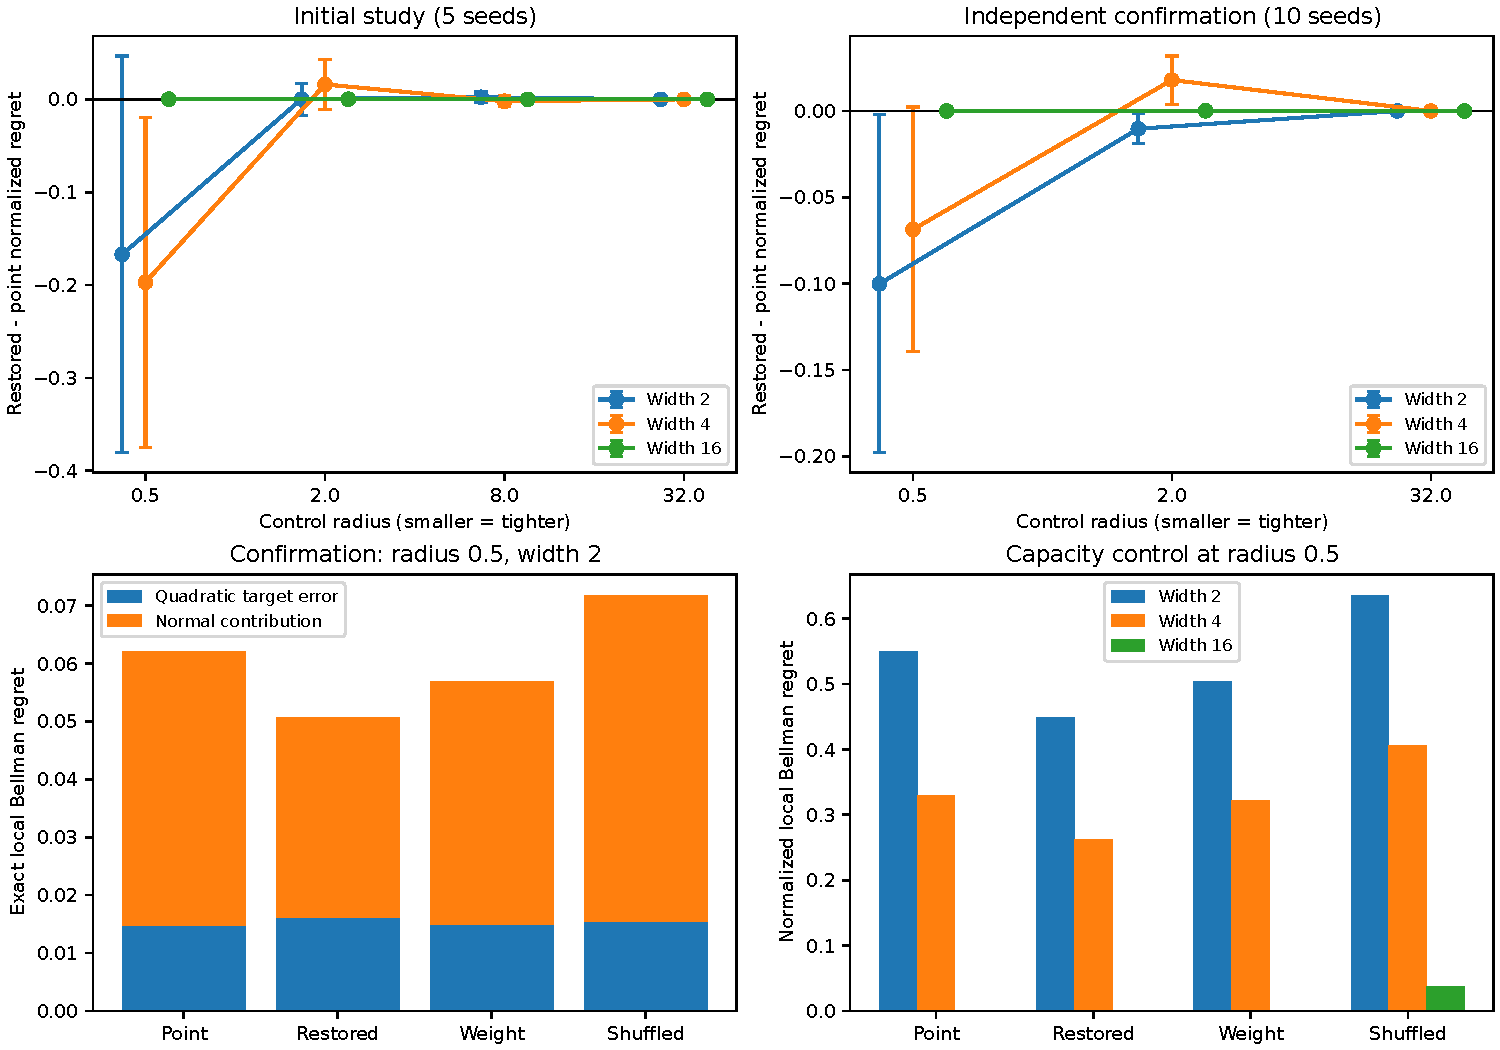
\includegraphics[width=\linewidth]{figures/neural_information_transfer.pdf}
 \caption{Top: restored-minus-point local regret and paired 95\% $t$
 intervals for the initial and independent samples. Bottom: confirmation
 loss decomposition on held-out teacher states and capacity response.}
 \label{fig:neural-information}
\end{figure}


Figure~\ref{fig:paired-effects} shows all ten confirmation-primary
paired effects. Their mean is $-0.10011$ and median $-0.03639$; the
two largest reductions account for 71.8\% of the summed reduction.
All signs favor restoration, but the typical paired effect is smaller
than the mean. The prespecified mean and its interval remain the
primary analysis; this descriptive plot exposes heterogeneity.
\begin{figure}[htbp]\centering
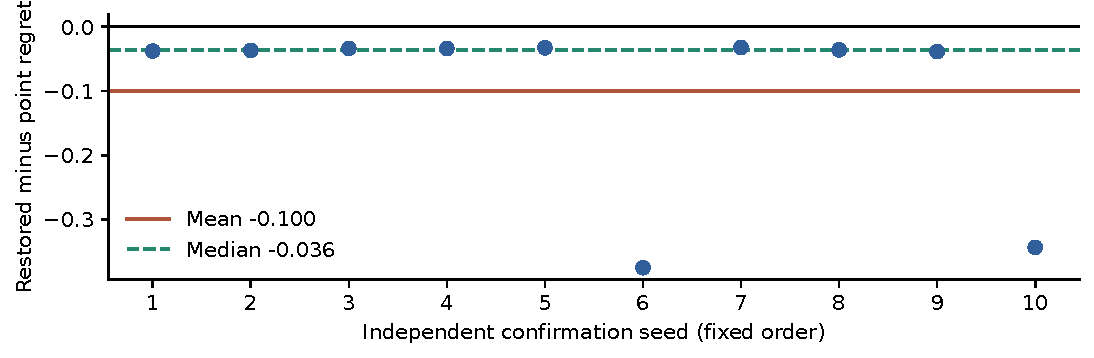
\includegraphics[width=.93\linewidth]{figures/neural_paired_effects.pdf}
\caption{All ten independent confirmation-primary paired differences
in normalized Bellman regret. Lines mark the mean and median.}
\label{fig:paired-effects}
\end{figure}
